\documentclass[11pt, letterpaper]{article} % Copyright (c) 2020 Brian Schubert


\def\LABnumber{}
\def\LABtitle{Design of a Simple 4-bit Processor}
\def\LABdatedue{August 18th, 2020}
\def\LABdatesubmitted{August 16th, 2020}
\def\LABabstract{\small In this project, we implement a 4-bit ALU supporting four arithmetic and logic functions: addition, subtraction, bitwise ``AND,'' and bitwise ``OR.'' The functionality of the ALU was verified both by  using the simulation tools provided by Quartus and by mapping it onto the DE1-SoC board's FPGA.}


% ECEE 2160 Lab Report Header
%
% Copyright (c) 2020 Brian Schubert
% 
% This header file was created to format lab reports in my
% Embedded Design course taken Northeastern University during
% the Summer 2 2020 semester.
%

% Many packages are retained from previous lab report headers
% for future convenience. 
\usepackage{amsmath,amsfonts,amssymb,amsthm}
\usepackage[english]{babel}
\usepackage{caption}
\usepackage[makeroom]{cancel}
\usepackage[dvipsnames,table]{xcolor}
\usepackage[inline]{enumitem}
\usepackage{esint}
\usepackage{fancyhdr}
\usepackage{geometry}
\usepackage{graphicx}
\usepackage{hyperref}
\usepackage[utf8]{inputenc}
\usepackage{listings} % For code listings
% Replace times with this package to typeset math in times aswell
% Note: no bold typeface exists for the times font, so \boldsymbol
% does not work when using a times font in math mode.
%\usepackage{mathptmx}
\usepackage{mathtools}
\usepackage{multicol}
\usepackage{multirow}
\usepackage{pgfplots}
\usepackage{placeins} % For FloatBarrier
\usepackage{siunitx}
\usepackage{subcaption}
\usepackage{tikz}
\usepackage[american]{circuitikz}
\usepackage{todonotes}
\usepackage{times} % For times font
\usepackage[explicit]{titlesec}

% Use deja-vu sans mono for monospaced typeface
% Must be after times font package.
\usepackage[scaled=0.9]{DejaVuSansMono}

\geometry{left=1in,right=1in,top=1in,bottom=1in}

% File prefixes to use when searching for graphics.
\graphicspath{ {../images/} {./images/} }

% Color all used links blue.
\hypersetup{
    colorlinks=true,
    linkcolor=MidnightBlue,   
    citecolor=MidnightBlue,   
    urlcolor=MidnightBlue,
}

\urlstyle{same} % Print URLs using the surroudning font instead of forcing monospace

% Add headings from lab report template
\pagestyle{fancy}
\lhead{\LABauthor\\\LABcourse}
\rhead{\LABcoursetitle\\Lab Assignment \LABnumber}

% Macro to generate the an IPL template style title page
\newcommand{\makelabtitle}{
\begin{titlepage}
    \begin{center}
    \renewcommand{\baselinestretch}{1.2}
    
    % See https://tex.stackexchange.com/questions/252040/unwanted-border-around-the-image
    % for details on how to fix border due transparent cropped region in png.
    
\includegraphics[width=0.7\textwidth]{northeastern-header-cropped}\par
    
    \vspace{0.6in}

    {
        \renewcommand{\baselinestretch}{1.2}
        \Large
        \LABcourse\par
        \LABcoursetitle\par
        \LABsemester\par
    }

    \vspace{0.3in}

    {\LARGE\bfseries
       \LABreportheading{} \LABnumber\par
        \ifx \LABtitle \undefined
        \else
            \LABtitle\par
        \fi
    }
    
    \vspace{0.3in}
    
    {
        \Large
        \LABauthor\par
        \ifx \LABauthoremail \undefined
        \else
            \large \texttt{\LABauthoremail}\par
        \fi
    }

    \vspace{0.4in}
    
    {
        \large
        \setlength{\tabcolsep}{4pt}
        \begin{tabular}{>{\bfseries}rl}
            Instructor:     & \LABinstructor\\
            Due Date: 	    & \LABdatedue\\
            Submitted:      & \LABdatesubmitted\\
        \end{tabular}
        
    }

    \end{center}
    \ifx \LABabstract \undefined
    \else
        \vfill\null
        \begin{abstract}
            \LABabstract
        \end{abstract}
    \fi
\end{titlepage}
}

% Common defaults for lab report title page
\def\LABcourse{ECEE 2160}
\def\LABcoursetitle{Embedded Design: Enabling Robotics}
\def\LABsemester{Summer 2 2020}
\def\LABauthor{Brian Schubert}
\def\LABauthoremail{schubert.b@northeastern.edu}
\def\LABinstructor{Syed Shazli}
\def\LABreportheading{Report for Lab Assignment}


% Notation Definitions
\newcommand{\dd}[1]{\mathrm{d}#1}
\newcommand{\diffop}[2][]{\frac{\dd#1}{\dd #2}}
\newcommand{\pdiffop}[2][]{\frac{\partial #1}{\partial #2}}
\newcommand{\bvec}[1]{{\vec{\boldsymbol{#1}}}}
\newcommand{\relerr}[1]{\frac{\delta #1}{#1}}
\newcommand{\unitvec}[1]{\hat{\boldsymbol{#1}}}

\sisetup{inter-unit-product =\cdot}
\sisetup{per-mode = symbol}
\sisetup{separate-uncertainty = true}
\sisetup{multi-part-units=single}
\DeclareSIUnit{\radian}{rad}
\DeclareSIUnit{\degreeFahrenheit}{{}^\circ F}

% Use computer modern roman fontface for emf symbol.
% https://tex.stackexchange.com/questions/67881/resetting-mathcal-font-to-default
\DeclareMathAlphabet{\defaultmathcal}{OMS}{cmsy}{m}{n}
\newcommand{\emf}{\defaultmathcal{E}}



% Print table and figure labels in bold font
\captionsetup[table]{labelfont=bf}
\captionsetup[figure]{labelfont=bf}

%\captionsetup[lstlisting]{ format=listing, labelfont=white, textfont=white, singlelinecheck=false, margin=0pt, font={bf,footnotesize} }
\captionsetup[lstlisting]{labelfont=bf}

% Make table columns slighly wider by default
\setlength{\tabcolsep}{8pt}

% Custom code color scheme
\definecolor{codekeyword}{RGB}{3,0,130}
\definecolor{codeidentifier}{RGB}{20, 20, 80}
\definecolor{codestring}{RGB}{72, 140, 2}
\definecolor{codecomment}{rgb}{0.3,0.3,0.3}
\definecolor{codedirective}{RGB}{160, 130, 60}


% Custom listings styling
\lstdefinestyle{labreportstyle}{
    % Syntax highlighting
    basicstyle=\ttfamily\footnotesize,
    backgroundcolor=\color{gray!5},
    commentstyle=\itshape\color{codecomment},
    keywordstyle=\bfseries\color{codekeyword},
    stringstyle=\bfseries\color{codestring},
    identifierstyle=\color{codeidentifier},
    % Tab width and display
    tabsize=4,
    showtabs=true,
    % Don't show spaces in strings
    showspaces=false,
    showstringspaces=false,
    % Show line numbers
    numbers=left,
    numberstyle=\scriptsize\sffamily\color{gray},
    % Allow listing to break long lines
    breaklines=true,
    breakatwhitespace=true,
    % Frame settings
    frame=lines,
%    frame=bottomline,
    % Misc
    captionpos=t,
    keepspaces=true,
    xleftmargin=2mm,
    framexleftmargin=2mm,
}

% C++ specific styling
\lstdefinestyle{labreportstyle-C++}{
    language=C++,	% Not sure if redundant now, but was required at one point
    style=labreportstyle,
    directivestyle={\color{codedirective}},
    morekeywords={constexpr,nullptr,noexcept,static\_assert,alignof}
%    frame=bottomline,
}

% shell specific styling
\lstdefinestyle{labreportstyle-sh}{
    language=sh,
    style=labreportstyle,
    numbers=none,
    identifierstyle=\color{black},
    emph={\$},
    emphstyle=\bfseries\color{codekeyword},
}

% Conveience macro to load code file listings.
%
% Note that the style is automatically selected based on the language paramater.
\newcommand{\includecode}[2][C++]{%
    \lstinputlisting[caption={\texttt{#2}}, label={lst:#2}, language=#1, style=labreportstyle-#1]{#2}
}

\def\LABreportheading{Final Project}
\rhead{\LABcoursetitle\\Final Project}

\usepackage{floatpag} % for thisfloatpagestyle
\usepackage{pdflscape}

\begin{document}
\makelabtitle

\section*{Introduction}

This project was an exercise in using Quartus to design combinational logic circuits.
A basic 4-bit arithmetic-logic unit (ALU) was designed using the Quartus block diagram editor. The ALU supported four operations: addition, subtraction, bitwise ``AND,'' and bitwise ``OR.''  The ALU circuit was mapped onto the DE1-SoC board's FPGA, and its behavior was verified by interacting with the board's I/O devices.

\section*{Lab Discussion}

\subsection*{Materials}

The following materials were used to complete this lab.
\begin{enumerate}
    \item Host computer (Linux Mint 19.3, x86\_64)
    \item DE1-SoC board (de1soclinux, armv7l)
\end{enumerate}
\subsection*{Software}
Intel's Quartus Prime Lite Edition (version 20.1) was installed on the host machine.



\section*{Results and Analysis}

This project consisted of designing a basic 4-bit ALU that supported the operations of addition, subtraction, bitwise ``AND'', and bitwise ``OR.'' A listing of the schematics produced for this project can be found in Table~\ref{tab:figure-summary} below.


The ALU circuit was tested using the Quartus Simulation Waveform Editor \cite{quartus-waveform-sim}. Test signals consisting of 1) a counter signal over integers from the interval $[0,15]$, and 2) randomly generated 4-bit integers were applied, respectively, to the two input groups  $A$ and $B$.  The results from the waveform simulations are provided in Figure~\ref{fig:wave-sims} below. Using the results of these simulations, the correctness of the ALU circuit could be verified by direct computation. All input combinations tested resulted in their expected outputs.

The ALU circuit was then loaded onto the DE1-SoC's FPGA board, with the input signals mapped to the board's switches and the output signal mapped to the board's LEDs. An index of the figures that demonstrate the ALU circuit's functionality on the DE1-SoC board is provided in Table~\ref{tab:figure-summary} below. All ALU functions behaved as expected on the DE1-SoC.

\begin{table}[h]\centering
    \caption{Summary of ALU Design and Test Figures.}\label{tab:figure-summary}
    \def\arraystretch{1.3}
    \begin{tabular}{cccc}
        \hline
        \textbf{ALU Function} & \textbf{Schematic} & \textbf{Waveform Test} & \textbf{Board Tests}\\
        \hline
        Adder & Figure~\ref{fig:schematic-4bit-adder} &  Figure~\ref{fig:wave-sims-adder} & Figures~~\hyperref[fig:board-test-adder]{\ref{fig:board-test-adder}a-c}\\
        Subtractor & Figure~\ref{fig:schematic-4bit-subtractor} &  Figure~\ref{fig:wave-sims-subtractor} & Figures~~\hyperref[fig:board-test-subtractor]{\ref{fig:board-test-subtractor}a-c}\\
        Bitwise ``AND'' & Figure~\ref{fig:schematic-4bit-int-and} &  Figure~\ref{fig:wave-sims-and} & Figures~\hyperref[fig:board-test-and]{\ref{fig:board-test-and}a-c}\\
        Bitwise ``OR'' & Figure~\ref{fig:schematic-4bit-int-or} &  Figure~\ref{fig:wave-sims-or} & Figures~\hyperref[fig:board-test-or]{\ref{fig:board-test-or}a-c}\\
        \hline
    \end{tabular}
\end{table}


\begin{figure}[h]
    \includegraphics[width=0.9\linewidth,clip,trim={7cm 20cm 2.8cm 2.8cm}]%
    {images/ecee2160_final_project.pdf}
    \caption{Schematic for basic 4-bit 4-function ALU.}\label{fig:schematic-alu}
\end{figure}

\begin{figure}[h]
    \includegraphics[width=0.9\linewidth,clip,trim={3cm 16.8cm 3cm 3cm}]%
    {images/ecee2160_final_project_4bit_adder.pdf}
    \caption{
        \centering Schematic for a 4-bit carry-lookahead adder.
        \newline (\texttt{ecee2160\_final\_project\_4\_bit\_adder})%
    }
    \label{fig:schematic-4bit-adder}
\end{figure}


\begin{figure}[h]
    \includegraphics[width=0.9\linewidth,clip,trim={5.5cm 20.3cm 3cm 3.8cm}]%
    {images/ecee2160_final_project_1bit_adder_lookahead.pdf}
    \caption{\centering Schematic for a 1-bit full-adder with propagate and generate outputs. 
        \newline(\texttt{ecee2160\_final\_project\_1bit\_adder\_lookahead})}
    \label{fig:schematic-1bit-adder}
\end{figure}

\begin{figure}[h]
    \includegraphics[width=0.9\linewidth,clip,trim={3cm 19.7cm 4cm 3cm}]%
    {images/ecee2160_final_project_4bit_int_and.pdf}
    \caption{\centering Schematic for a 4-bit integer AND gate. \newline
        (\texttt{ecee2160\_final\_project\_4bit\_int\_and})}
    \label{fig:schematic-4bit-int-and}
\end{figure}

\begin{figure}[h]
    \includegraphics[width=0.9\linewidth,clip,trim={3cm 19.7cm 4cm 3cm}]%
    {images/ecee2160_final_project_4bit_int_or.pdf}
    \caption{\centering Schematic for a 4-bit integer OR gate.\newline (\texttt{ecee2160\_final\_project\_4bit\_int\_or})}
    \label{fig:schematic-4bit-int-or}
\end{figure}

\begin{figure}[h]
    \includegraphics[width=0.9\linewidth,clip,trim={8cm 21.5cm 3cm 4.5cm}]%
    {images/ecee2160_final_project_4bit_subtractor.pdf}
    \caption{\centering Schematic for a 4-bit substractor.
        \newline(\texttt{ecee2160\_final\_project\_4bit\_subtractor})}
    \label{fig:schematic-4bit-subtractor}
\end{figure}


\begin{landscape}
\begin{figure}[p]\centering
    \def\figureSpacing{0.5cm}
    \thisfloatpagestyle{empty}
    \begin{subfigure}{\linewidth}\centering
        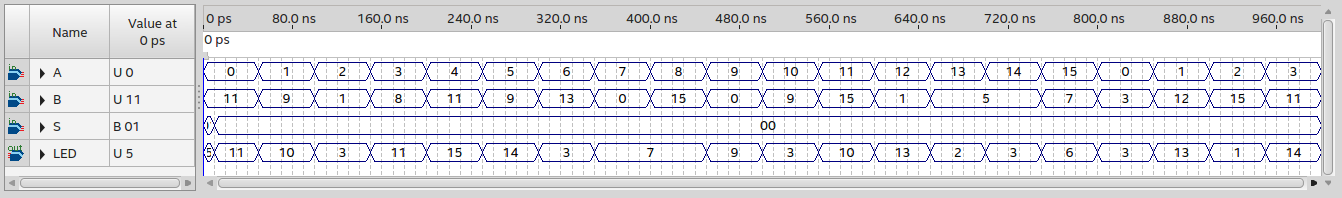
\includegraphics[width=0.9\linewidth]{images/sim-adder.png}
        \caption{4-bit addition results (\texttt{A+B}, values in unsigned decimal).}
        \label{fig:wave-sims-adder}
    \end{subfigure}
    \\[\figureSpacing]
    \begin{subfigure}{\linewidth}\centering
        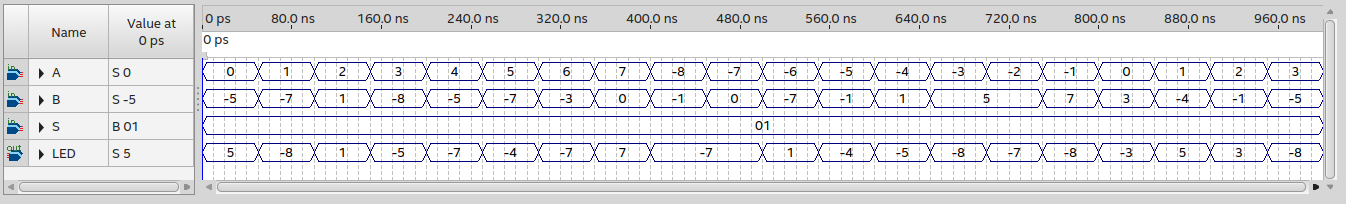
\includegraphics[width=0.9\linewidth]{images/sim-subtractor.png}
        \caption{4-bit subtraction results (\texttt{A-B}, values in signed decimal).}
        \label{fig:wave-sims-subtractor}
    \end{subfigure}
    \\[\figureSpacing]
    \begin{subfigure}{\linewidth}\centering
        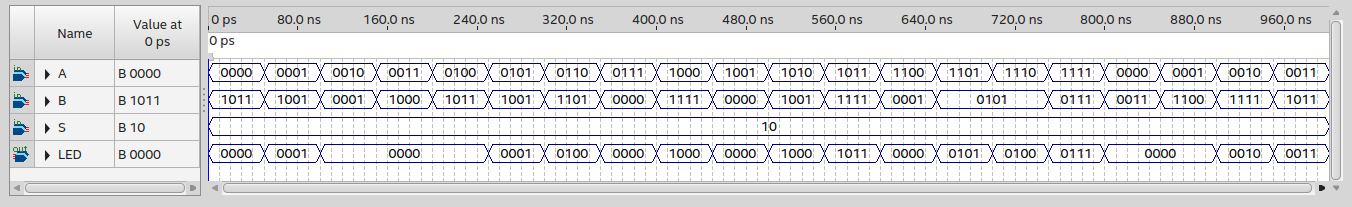
\includegraphics[width=0.9\linewidth]{images/sim-and.png}
        \caption{4-bit ``AND'' results (\texttt{A\&B}, values in binary).}
        \label{fig:wave-sims-and}
    \end{subfigure}
    \\[\figureSpacing]
    \begin{subfigure}{\linewidth}\centering
        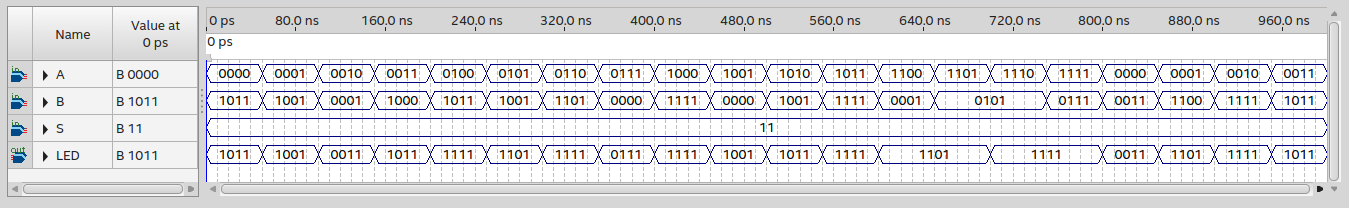
\includegraphics[width=0.9\linewidth]{images/sim-or.png}
        \caption{4-bit ``OR'' results (\texttt{A|B}, values in binary).}
        \label{fig:wave-sims-or}
    \end{subfigure}
    \caption{4-bit ALU simulation results in Quartus Simulation Waveform Editor.}\label{fig:wave-sims}
\end{figure}
\end{landscape}

\begin{figure}[p]\centering
    \begin{subfigure}{0.48\linewidth}\centering
        \fbox{\includegraphics[width=\linewidth,trim={10cm 6.5cm 8cm 11cm},clip]%
        {images/board_a3_plus_b1.JPG.pdf}}
        \caption{$3_{10} + 1_{10} = 4_{10}$.}
    \end{subfigure}
    \hfill\null
    \begin{subfigure}{0.48\linewidth}\centering
        \fbox{\includegraphics[width=\linewidth,trim={7.2cm 4.6cm 7cm 11.3cm},clip]%
            {images/board_a5_plus_b3.JPG.pdf}}
        \caption{$5_{10} + 3_{10} = 8_{10}$.}
    \end{subfigure}
    \\[4mm]
    \begin{subfigure}{0.48\linewidth}\centering
        \fbox{\includegraphics[width=\linewidth,trim={10cm 6.5cm 8cm 11cm},clip]%
        {images/board_a12_plus_b7.JPG.pdf}}
        \caption{$12_{10} + 7_{10} = 19_{10} \equiv 3_{10} \mod 16$.}
    \end{subfigure}
    \caption{\centering Addition using 4-bit ALU mapped onto the DE1-SoC's FPGA board. \newline (Pink--Input $A$, \quad Green--Input $B$, \quad Grey--Select $S$)}
    \label{fig:board-test-adder}
\end{figure}

\begin{figure}[p]\centering
    \begin{subfigure}{0.48\linewidth}\centering
        \fbox{\includegraphics[width=\linewidth,trim={7.2cm 4.6cm 7cm 11.3cm},clip]%
            {images/board_a1_minus_b2.JPG.pdf}}
        \caption{$1_{10} - 2_{10} = -1_{10}$.}
    \end{subfigure}
    \hfill\null
    \begin{subfigure}{0.48\linewidth}\centering
        \fbox{\includegraphics[width=\linewidth,trim={10cm 6.5cm 8cm 11cm},clip]%
            {images/board_a-5_minus_6.JPG.pdf}}
        \caption{Subtractor: $-5_{10} - 6_{10} = -11 \equiv 5_{10} \mod 16$.}
    \end{subfigure}
    \\[4mm]
    \begin{subfigure}{0.48\linewidth}\centering
        \fbox{\includegraphics[width=\linewidth,trim={10cm 6.5cm 8cm 11cm},clip]%
            {images/board_a-5_minus_b-2.JPG.pdf}}
        \caption{Subtractor: $-5_{10} - (-2_{10}) = -3$.}
    \end{subfigure}
    \caption{\centering Subtraction using 4-bit ALU mapped onto the DE1-SoC's FPGA board. \newline (Pink--Input $A$, \quad Green--Input $B$, \quad Grey--Select $S$)}
    \label{fig:board-test-subtractor}
\end{figure}

\begin{figure}[p]\centering
    \begin{subfigure}{0.48\linewidth}\centering
        \fbox{\includegraphics[width=\linewidth,trim={7.2cm 4.6cm 7cm 11.3cm},clip]%
            {images/board_a1000_and_b1111.JPG.pdf}}
        \caption{$1000_2 \land 1111_2 = 1000_2$.}
    \end{subfigure}
    \hfill\null
    \begin{subfigure}{0.48\linewidth}\centering
        \fbox{\includegraphics[width=\linewidth,trim={7.2cm 4.6cm 7cm 11.3cm},clip]%
            {images/board_a1111_and_b1000.JPG.pdf}}
        \caption{$1111_2 \land 1000_2 = 1000_2$.}
    \end{subfigure}
    \\[4mm]
    \begin{subfigure}{0.48\linewidth}\centering
        \fbox{\includegraphics[width=\linewidth,trim={10cm 6.5cm 8cm 11cm},clip]%
            {images/board_a1101_and_b1011.JPG.pdf}}
        \caption{$1101_{2} \land 1011_{2} = 1001_{2}$.}
    \end{subfigure}
   \caption{\centering Bitwise ``AND'' using 4-bit ALU mapped onto the DE1-SoC's FPGA board. \newline (Pink--Input $A$, \quad Green--Input $B$, \quad Grey--Select $S$)}
   \label{fig:board-test-and}
\end{figure}

\begin{figure}[p]\centering
     \begin{subfigure}{0.48\linewidth}\centering
        \fbox{\includegraphics[width=\linewidth,trim={7.2cm 4.6cm 7cm 11.3cm},clip]%
             {images/board_a0011_or_b0110.JPG.pdf}}
        \caption{$0011_2 \lor 0110_2 = 0111_2$.}
    \end{subfigure}
    \hfill\null
     \begin{subfigure}{0.48\linewidth}\centering
         \fbox{\includegraphics[width=\linewidth,trim={7.2cm 4.6cm 7cm 11.3cm},clip]%
             {images/board_a1111_or_b0000.JPG.pdf}}
         \caption{$1111_2 \lor 0000_2 = 1111$.}
     \end{subfigure}
     \\[4mm]
     \begin{subfigure}{0.48\linewidth}\centering
         \fbox{\includegraphics[width=\linewidth,trim={10cm 6.5cm 8cm 11cm},clip]%
             {images/board_a0101_or_b0011.JPG.pdf}}
         \caption{$0101_{2} \lor 0011_{2} = 0111_{2}$.}
     \end{subfigure}
     \caption{\centering Bitwise ``OR'' using 4-bit ALU mapped onto the DE1-SoC's FPGA board. \newline (Pink--Input $A$, \quad Green--Input $B$, \quad Grey--Select $S$)}
     \label{fig:board-test-or}
\end{figure}


\FloatBarrier
\section*{Conclusion}

This lab illustrated the process of designing large combinational circuits by combining smaller logical units. Basic 4-bit adder, subtractor, bitwise ``AND,'' and bitwise ``OR''  circuits were implemented using Quartus and combined to produce a simple arithmetic-logic unit. The ALU circuit was tested both by using simulation software and by mapping it onto a FPGA board.  Common issues when designing combinational circuits such as power consumption and propagation delay were considered and addressed during this project. 

This project could be extended either by increasing the word size of the ALU or by introducing additional arithmetic functions. Additionally, for this project, no requirements were imposed on the design of the arithmetic circuits other than their terminal behavior. Therefore this lab might be further extended by introducing constraints to the circuit design process such as minimizing time complexity or power consumption.

\FloatBarrier

\nocite{quartus-schematics}
\nocite{fell-discrete-structure}
\bibliography{../ecee-2160-common.bib,./ecee-2160-alu-project.bib}

\bibliographystyle{unsrt}

\end{document}